\begin{figure}[t]
    \centering
    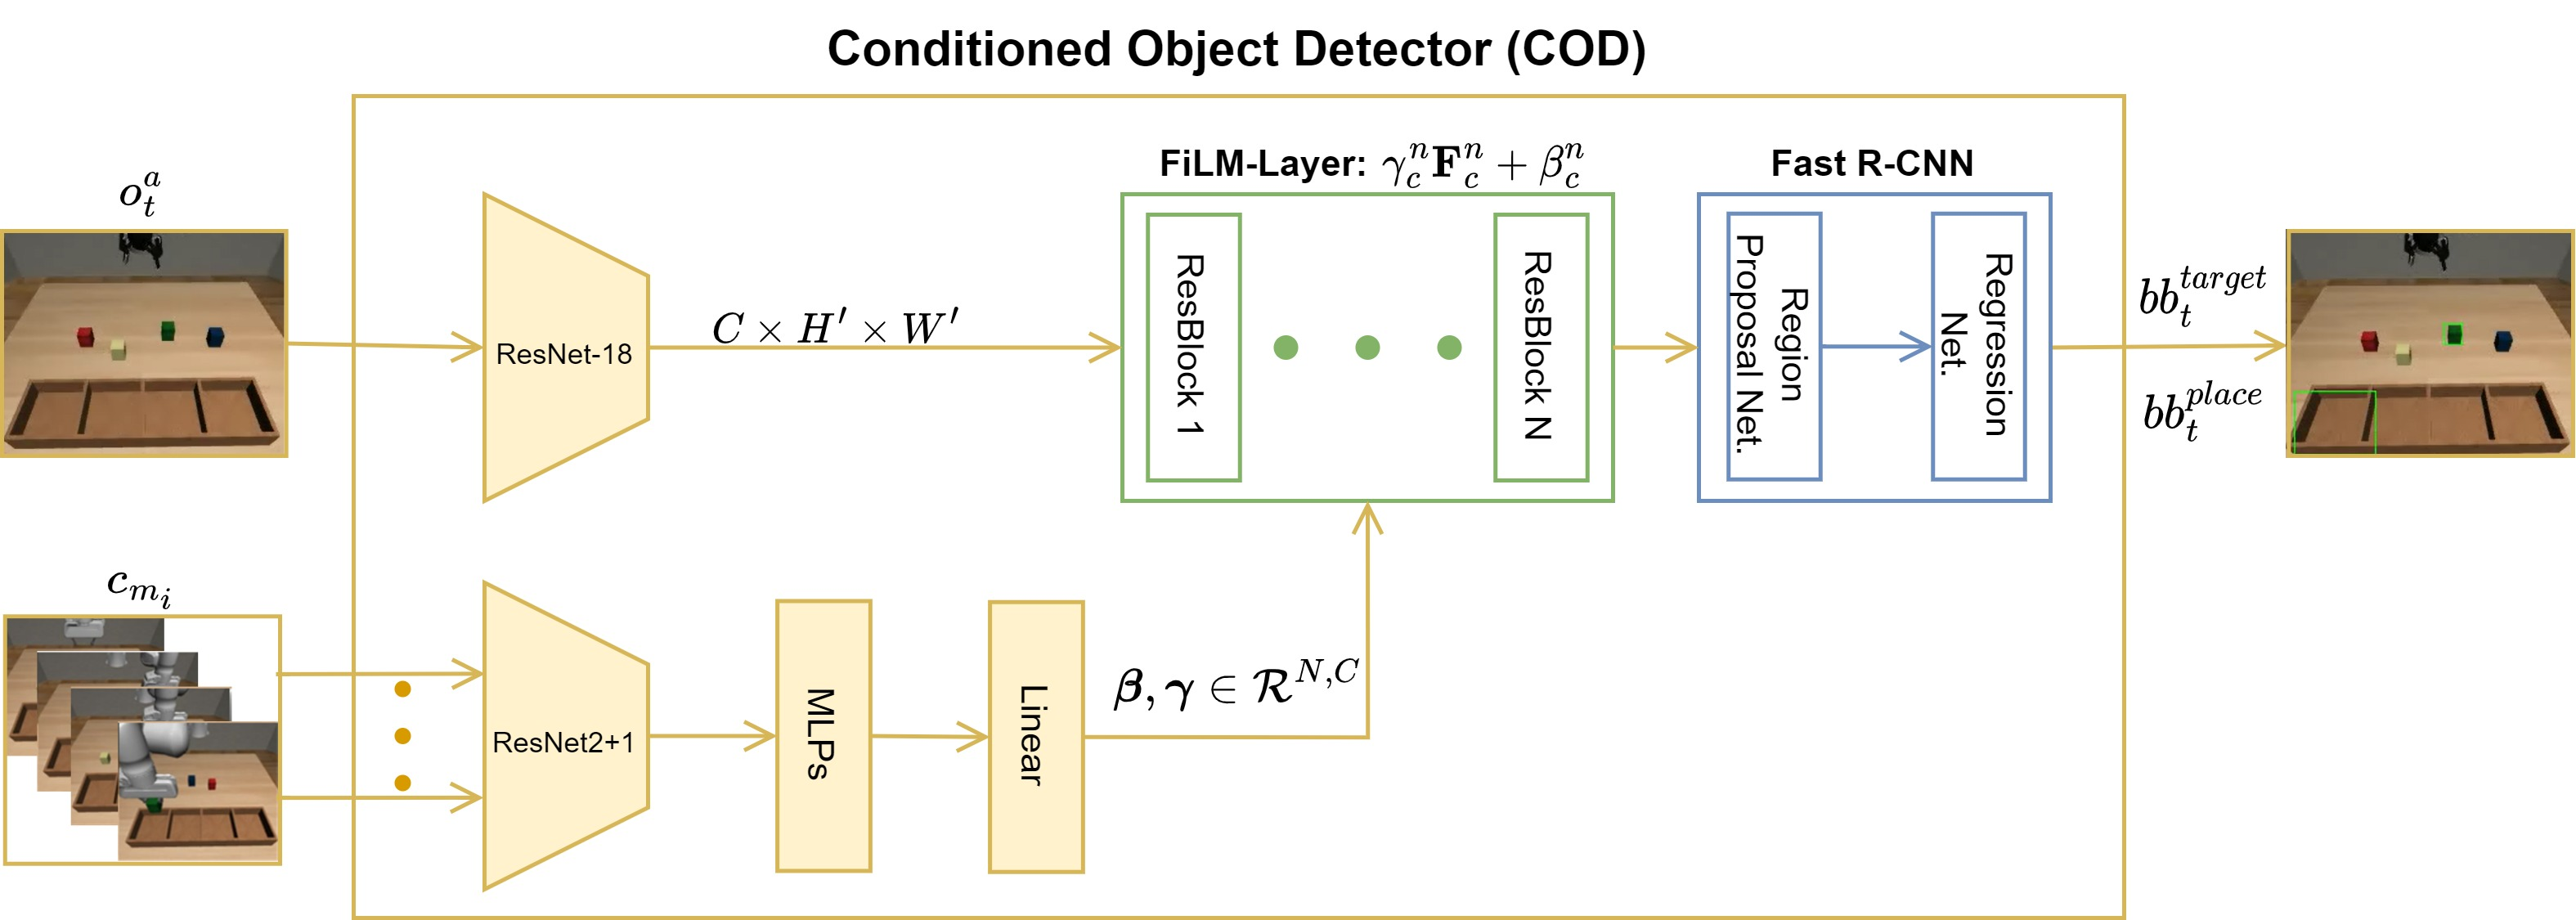
\includegraphics[width=1.0\textwidth]{figures/images/ch2/cod.jpg}
    \caption{The proposed \textit{Conditioned Object Detector} architecture takes as input the pair $(o^{a}_{t}, c_{m_{i}})$, where $o^{a}_{t}$ represents the agent observation and $c_{m_{i}}$ represents the demonstration frames. The agent observation is encoded using ResNet-18, while the demonstration frames are encoded through ResNet2+1. The FiLM conditioning layer is employed to inject information from the command $c_{m_{i}}$ into the feature maps extracted from the observation. Finally, Fast R-CNN generates the bounding boxes based on the conditioned input.}
    \label{fig:cod}
\end{figure}
